\section{Two-dimensional disks with beta cooling}\label{result_2d}
We begin in the 2D limit with beta cooling  to make connection 
with previous studies. The disk
material is assumed to be confined to the midplane so $\delta v_z=0$. 
We make the replacement  
$\rho \to \Sigma$, re-interpret $P$ as the vertically-integrated
pressure, and set $\Gamma=1$ without loss of generality. 
The gravitational potential perturbation remains 3D and its midplane
value is given by    
\begin{align}
  \delta \Phi(z=0) = -\frac{2 \pi G}{|k|}\delta\Sigma
\end{align}
\citep{shu70}.
 
The linearized equations yield an algebraic dispersion relation $s =
s(k)$. We write this  
in terms of the dimensionless growth rate $S = s/\Omega$ and
wavenumber $K=kH = k c_{s0}/\Omega$ as
\begin{align}\label{thindisk}
  f(S,K)\equiv AD - BC = 0,   
\end{align}
where the functions $A,B,C,D$ are given in Appendix \ref{2ddisp}. 

\subsection{Inviscid limit}\label{2d_inviscid}
Here we neglect viscosity by setting 
$\alpha = \alpha_b = 0$. This eliminates viscous GI and 
allows us to quantify the \emph{sole} effect of cooling on the
perturbations. An external, time-independent heat source should be
invoked to balance the imposed cooling to allow an equilibrium to be
defined ($\mathcal{H}_\mathrm{ext}\neq 0$). Alternatively, we are
assuming viscosity only provides a background heating and does not
play an active role in the perturbed state. %may or may not be true in a real
                                %disk because we are using viscosity
                                %as proxy for turbulence

Eq. \ref{thindisk} simplifies to  
\begin{align}\label{inviscid}
%  &\beta S^3 + S^2 - \beta \left\{ \frac{2|K|}{\qtwo} - \left[2(2-q) +
%    \gamma K^2\right]\right\}S \notag\\ &- \left[\frac{2|K|}{\qtwo} - 2(2-q)\right]
%  = 0. 
  S^2 = \frac{2|K|}{Q} - 2(2-q) - \left(\frac{\theta + \beta \gamma
    S}{1+\beta S}\right)K^2, 
\end{align}
similar to the classic Lin-Shu dispersion relation, which may be
obtained by taking the limit $|\beta S|\to\infty$. 
The first term on
the right-hand-side represents destabilization by self-gravity; 
the second and third terms represent stabilization by rotation and
pressure, respectively. The imposed cooling only affects the
pressure response. 

Eq. \ref{inviscid} is a cubic equation in $S$. The 
Routh-Hurwitz criteria imply that stability is ensured if 
\begin{align}\label{stable_condition}
  \gamma > \theta \quad \text{and} \quad 
  Q > \frac{1}{\sqrt{2\theta(2-q)}} 
\end{align}
are both satisfied. Thus, whether or not the system is stable is
independent of the cooling rate $\beta$ (provided it is non-zero and
finite). The system becomes more unstable with decreasing $\theta$.   

Consider the most unstable wavenumber $|K_*|$ at which $\p S/\p |K| =
0$ and $S = 
S_*$. By differentiating Eq. \ref{inviscid}, we obtain 
\begin{align}\label{kstar}
%  |K_*| = \frac{1}{\gamma \qtwo} \left(1 + \frac{1}{\beta S_*}\right). 
  |K_*| = \frac{1+\beta S_*}{Q\left(\theta + \gamma \beta S_*\right)}
\end{align}
%Eq. \ref{kstar} describes how the most unstable  mode is affected by
%cooling ($\beta$) and external heating ($\theta$). 
Inserting this into Eq. \ref{inviscid}, we find the maximum growth
rate satisfies
\begin{align}\label{inviscid_max}
%  S_*^3 + \left[2(2-q)  - \frac{1}{\gamma \qtwo^2}\right]S_* - \frac{1}{\gamma
%    \qtwo^2 \beta} = 0.
  S_*^2 = \frac{1+\beta S_*}{Q^2\left(\theta + \beta\gamma S_*\right)}
  - 2(2-q).
\end{align}
General solutions to this cubic for $S_*$ are unwieldy, but simple
results may be obtained in special cases, discussed next. 


\subsubsection{$\theta = 0$}\label{theta0}
%Beta cooling with $\theta=0$ is commonly employed in 
%numerical simulations of self-gravitating disks \citep{gammie01}. 
For beta cooling with $\theta=0$, the disk is unconditionally
unstable for finite $Q$. The most unstable wavelength decreases with
decreasing $\beta$. The $\beta\to0$ limit corresponds to a
pressureless disk (not merely isothermal).   


Let us consider a disk with 
\begin{align}\label{qcrit_def}
  \qtwo = \frac{1}{\sqrt{2\gamma(2-q)}}\equiv Q_{\mathrm{crit}},
\end{align} 
so that it is marginally stable in the absence of cooling.  
How does finite cooling destabilize the disk?  
Inserting Eq. \ref{qcrit_def} into Eq. \ref{inviscid_max} and setting
$\theta=0$, we find 
%In this case the coefficient of 
%$S_*$ in Eq. \ref{inviscid_max} vanish, so that  
\begin{align}\label{sstar}
  S_*^3 = \frac{1}{\gamma Q_\mathrm{crit}^2 \beta}. 
\end{align}
The maximum growth rate, $S_*\propto \beta^{-1/3}$, smoothly
increases with decreasing $\beta$. Instability does not require the
cooling time to be below some critical value. 

Nevertheless, we can define a characteristic cooling
time $\beta_*$ as that which removes pressure support against
self-gravity over the natural lengthscale in the problem, $H$. We
thus set $|K_*|=1$ and find, for the Keplerian disk, 

\begin{align}\label{betastar}
  \beta_* = \frac{1}{\left(\sqrt{\gamma} - 1\right)^{3/2}}. 
\end{align}
%Table \ref{bstar_compare} compares Eq. \ref{betastar} to 
%previously reported values of $\beta_c$ 
%for which fragmentation
%occurs.
This $\beta_*$ is similar to values of the cooling times, $\beta_\mathrm{c}$,
below which fragmentation occur on dynamical timescales in
numerical simulations of self-gravitating disks
\citep{gammie01,rice05,rice11}, which employ the same beta cooling prescription.    
We compare these in Table \ref{bstar_compare}, showing rough
agreement; and further discuss the potential significance of this result in
\S\ref{prev_works}. 

%{\bf brief physical interpretation. gravito-turbulent heating is a
%  constant background heating - it does not affect perturbations about
%  the turbulent state.  
%  imposed beta cooling works on all
%  scales. but `gravito-turbulence' only makes sense on scales larger
%  than averaging procedure (probably about $H$). }
%{\bf wild guess: fragmentation had high resolution because internal
%  structure of forming-clumps become resolved. internal turbulence
%  helps collapse. 
%}

\begin{deluxetable}{rrrr}
  \tablecolumns{4}
  \tablecaption{Characteristic cooling times as a function of
    $\gamma$. \label{bstar_compare}
  }
  \tablehead{
    %\colhead{}    &  \multicolumn{3}{c}{Non-shell Stars} &   \colhead{}   &
    %\multicolumn{3}{c}{Shell Stars} \\
    %\cline{2-4} \cline{6-8} \\
    \colhead{$\gamma$}   & \colhead{Eq. \ref{betastar}, $\beta_*$} &
    \colhead{Simulation, $\beta_c$} &  \colhead{Reference}
  }
\startdata
 $7/5$ & 12.75 & 12---13 & \cite{rice05}\\
$1.6$  &  7.33 & 8 & \cite{rice11}\\
$5/3$  &  6.37 & 6---7 & \cite{rice05}\\
$2$    &  3.75 & 3 & \cite{gammie01}
\enddata
\end{deluxetable}

\subsubsection{$\theta = 1$}\label{theta1}
Beta cooling with $\theta=1$ corresponds to 
`thermal-relaxation' in a strictly inviscid disk: the temperature is restored to its initial
value over the cooling time \citep{lin15,mohandas15}. In this case 
$\beta\to 0$ corresponds to an isothermal disk and $\beta
\to \infty$ corresponds to an adiabatic disk. (These two limits are
equivalent for $\gamma=1$.) The most unstable wavenumber and growth
rates vary weakly with $\beta$.   

%nothing interesting here 

%\subsubsection{Expected maximum stress}
%{\bf for notes only} 
%A reasonable assumption is that in the non-linear regime 
%there is an associated turbulent viscosity that may be estimated  
%as $\nu \sim l^2s$, where the lengthscale $l\sim 1/k$; which
%translates to $\alpha\sim S/K^2$.  
%
%Using Eq. \ref{pressureless}, we find that 
%\begin{align}\label{max_alpha}
%  \mathrm{max}\left(\frac{S}{K^2}\right) = \frac{3^{3/2}}{2^{7/2}\left(2-q\right)^{3/2}Q^2}
%\end{align}
%in the limit $\beta\to 0$. This maximum is occurs at wavenumber $|K| =
%4Q(2-q)/3$, which is $O(1)$ for typical disk parameters we consider. 
%Eq. \ref{max_alpha} indicates that $\alpha\propto Q^{-2}$, as
%suggested by \cite{lin87}. Note that although
%$\mathrm{max}(S)\to\infty$ as $\beta\to0$ (Eq. \ref{sstar}), 
%the associated stress is bound because the
%most unstable modes occur at the smallest scales. In fact, for
%$Q=Q_\mathrm{crit}$, we find $s(K_*)/K_*^2 \propto \beta $ as
%$\beta\to 0$, so transport by the most unstable mode is expected to be
%unimportant. 
%\begin{figure}
%  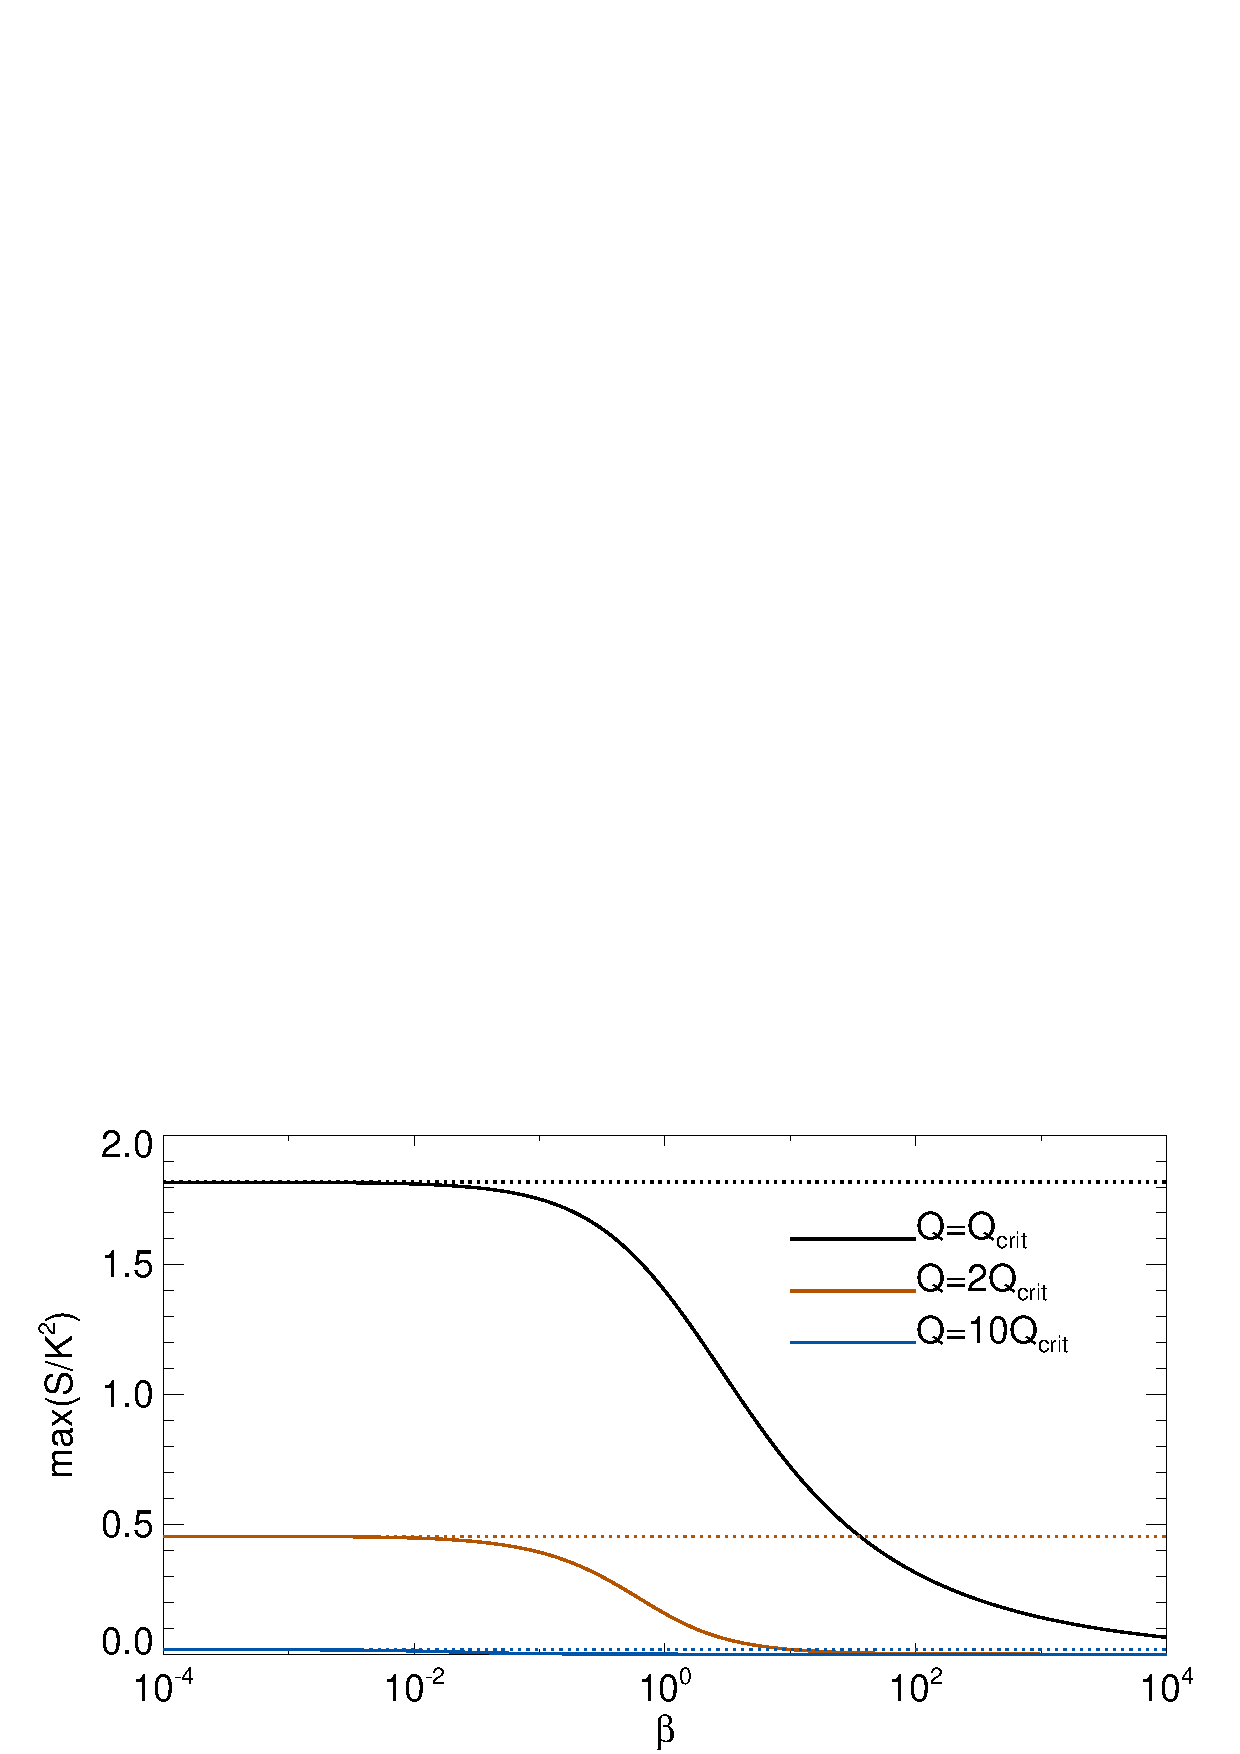
\includegraphics[width=\linewidth,clip=true,trim=0cm 0cm 0cm 0.8cm]{figures/inviscsg_alpha}
%  \caption{A measure of the
%    associated stress that can be expected in the non-linear
%    regime. The horizontal dotted lines
%    correspond to Eq. \ref{max_alpha}.}
%\end{figure}

\subsection{Viscous disk}\label{2dvisc}
We now consider a viscous disk with 
$\mu=-1,\,\lambda=0$ as discussed in \S\ref{visc_model}. We first
check in Appendix \ref{gammie_check} that our dispersion relation
reduces previous results in the adiabatic/isothermal limit.  

To see the effect of finite cooling, we simplify the dispersion relation,
Eq. \ref{thindisk}, by assuming $|\beta S|\ll 1$. Then  
for $|K| \to 0$ we find
\begin{align}\label{gammie_smallk}
%  S \sim \frac{\alpha |K|^3}{(2-q)Q},%derived assuming |beta*S|<<1 
%  S \sim \frac{\alpha K^2\left[2|K|Q^{-1} - \gamma K^2 + 2\alpha q
%    (2-q)(\gamma-1)K^2\right]}{2(2-q)+\gamma K^2 - 2|K|Q^{-1}} %derived
                                %assuming |\beta S|>>1
  S\simeq \frac{\alpha K^2}{2(2-q)}\left(\frac{2|K|}{Q} - \theta
  K^2\right), 
\end{align}
which coincides with \citeauthor{gammie96}'s Eq. 18 for vanishing
wavenumber. For $|K|\to\infty$ we find
\begin{align}\label{gammie_bigk}
  %  S \sim \frac{2}{Q|K|}\left(\frac{4}{3}\alpha + \gamma\beta\right)^{-1}.
  S \simeq\left(\frac{2}{Q|K|} - \theta\right)\left(\frac{4}{3}\alpha + 
  \alpha_b + \gamma\beta\right)^{-1}.
\end{align}



For $\theta\ll1$ a rough measure of the maximum growth rate can be obtained by
equating Eq. \ref{gammie_smallk} and \ref{gammie_bigk}\footnote{If
  $\theta$ is not small and/or $Q$  is large then one may just use Eq. \ref{gammie_smallk}
  to maximize $S$ over $K$, see the $\theta=0.3,\beta=100$ curve in the bottom
  panel of Fig. \ref{gammie_rate_plot}}.  
This exercise yields 
\begin{align}\label{gammie_maxrate_simple}
  %S_* \simeq
  %\frac{1}{Q}\left(\frac{\alpha}{2-q}\right)^{1/4}\left(\frac{6}{4\alpha
%+ 3\gamma\beta}\right)^{3/4}. 
  S_*\simeq \frac{
    6^{3/4}\left[\alpha\left(4\alpha +
      3\alpha_b + 3\gamma\beta\right)\right]^{1/4} - 3\theta
    Q(2-q)^{1/4}}{Q\left(4\alpha + 3\alpha_b +
    3\gamma\beta\right)(2-q)^{1/4}}. 
\end{align} 
%gravito-viscous instability 

As a numerical example, we consider a model with $\alpha_b=0$ and
$\alpha=\alpha(\beta)$ given by thermal equilibrium (
Eq. \ref{alpha_beta_relation}). Furthermore, we relate 
\begin{align}
  Q = \frac{Q_\mathrm{crit}}{\sqrt{\alpha}},\label{Qalpha}
\end{align}
to mimic a basic state maintained by gravito-turbulence where one
might expect the dimensionless stress $\alpha \sim Q^{-2}$
\citep{lin87}.   

Fig. \ref{gammie_rate_plot} show growth rates as a function of the
wavenumber $k$ obtained from the dispersion relation
Eq. \ref{thindisk}. The limiting behavior for small/large $K$ are
well-captured by Eq. \ref{gammie_smallk} and
\ref{gammie_bigk}. Comparing the two panels shows that increasing the
irradiation level ($\theta$) surpresses small-scale perturbations.     

\begin{figure}
  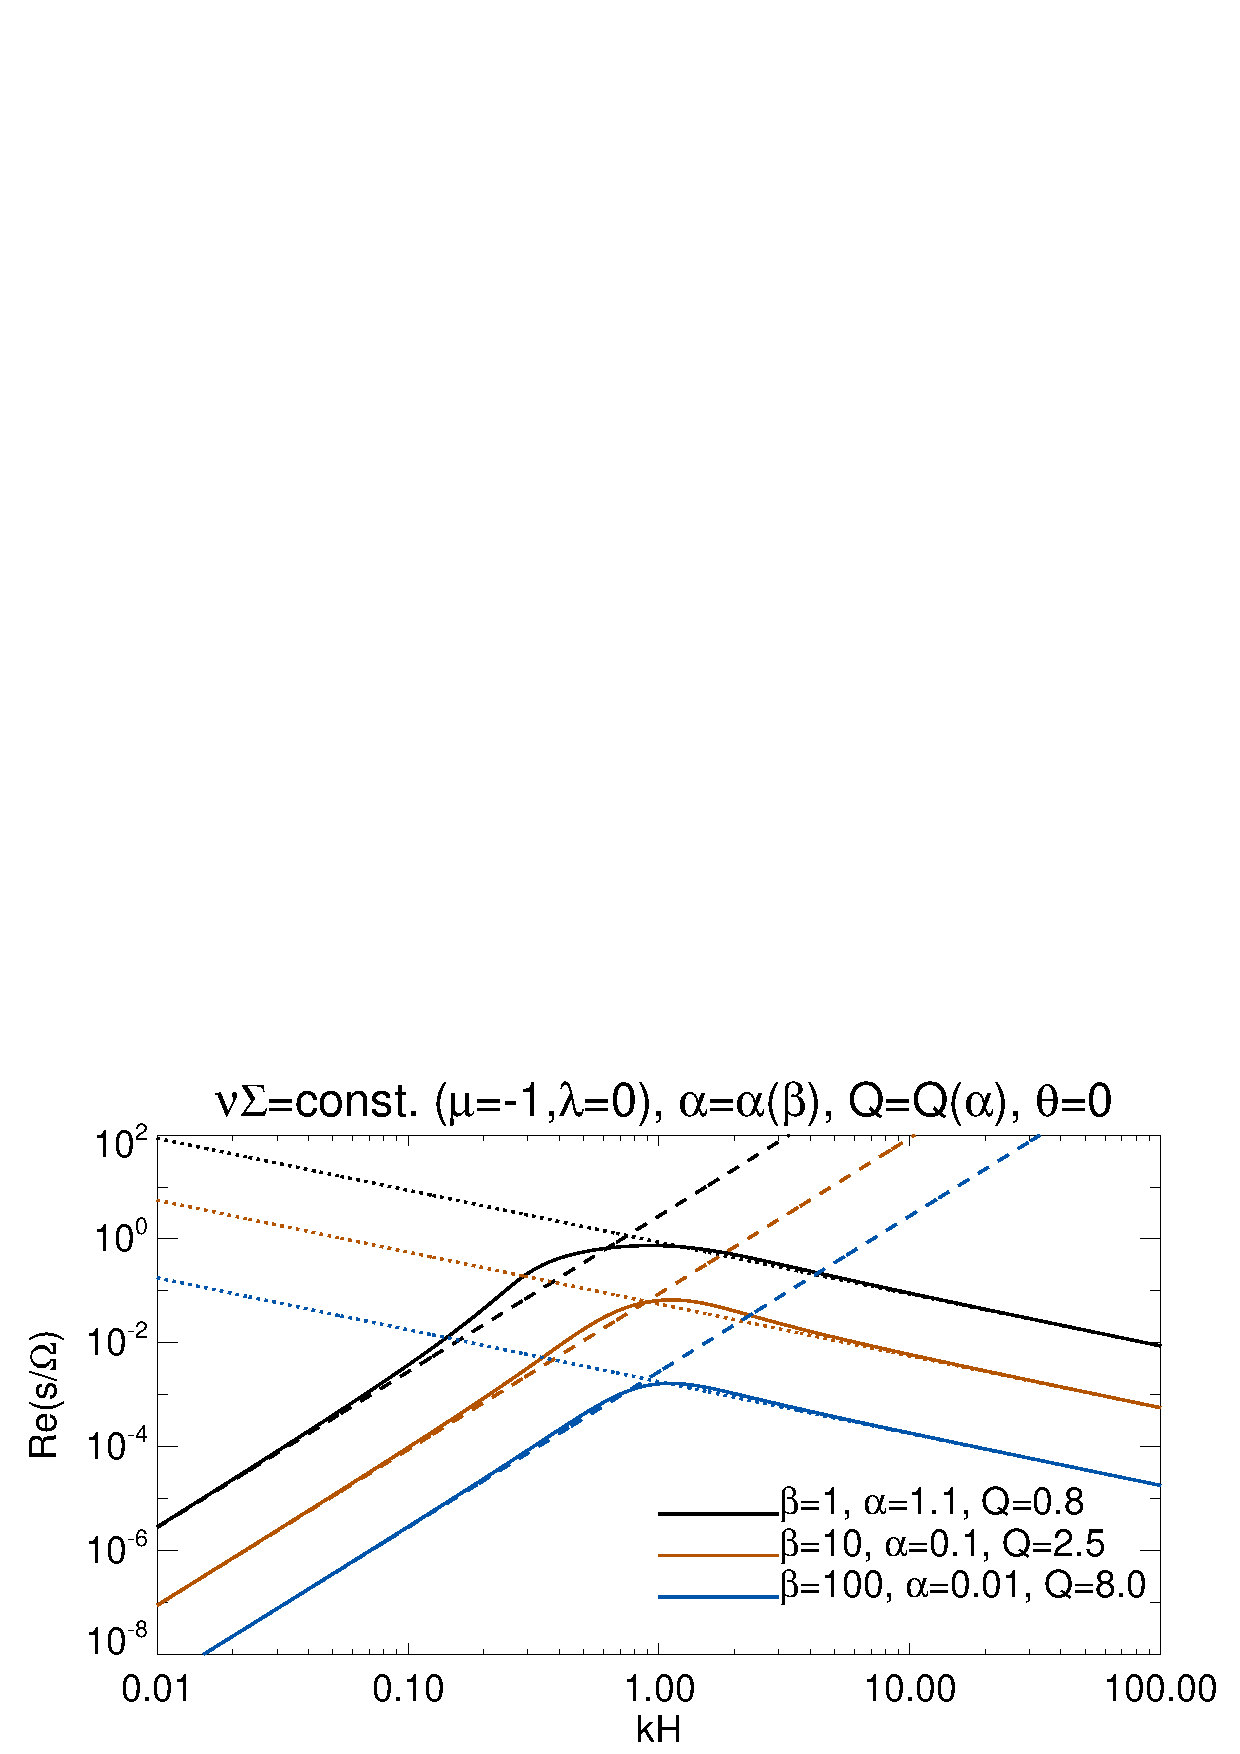
\includegraphics[width=\linewidth,clip=true,trim=0cm 1.5cm 0.4cm
    0.0cm]{figures/viscsg_modes}\\
  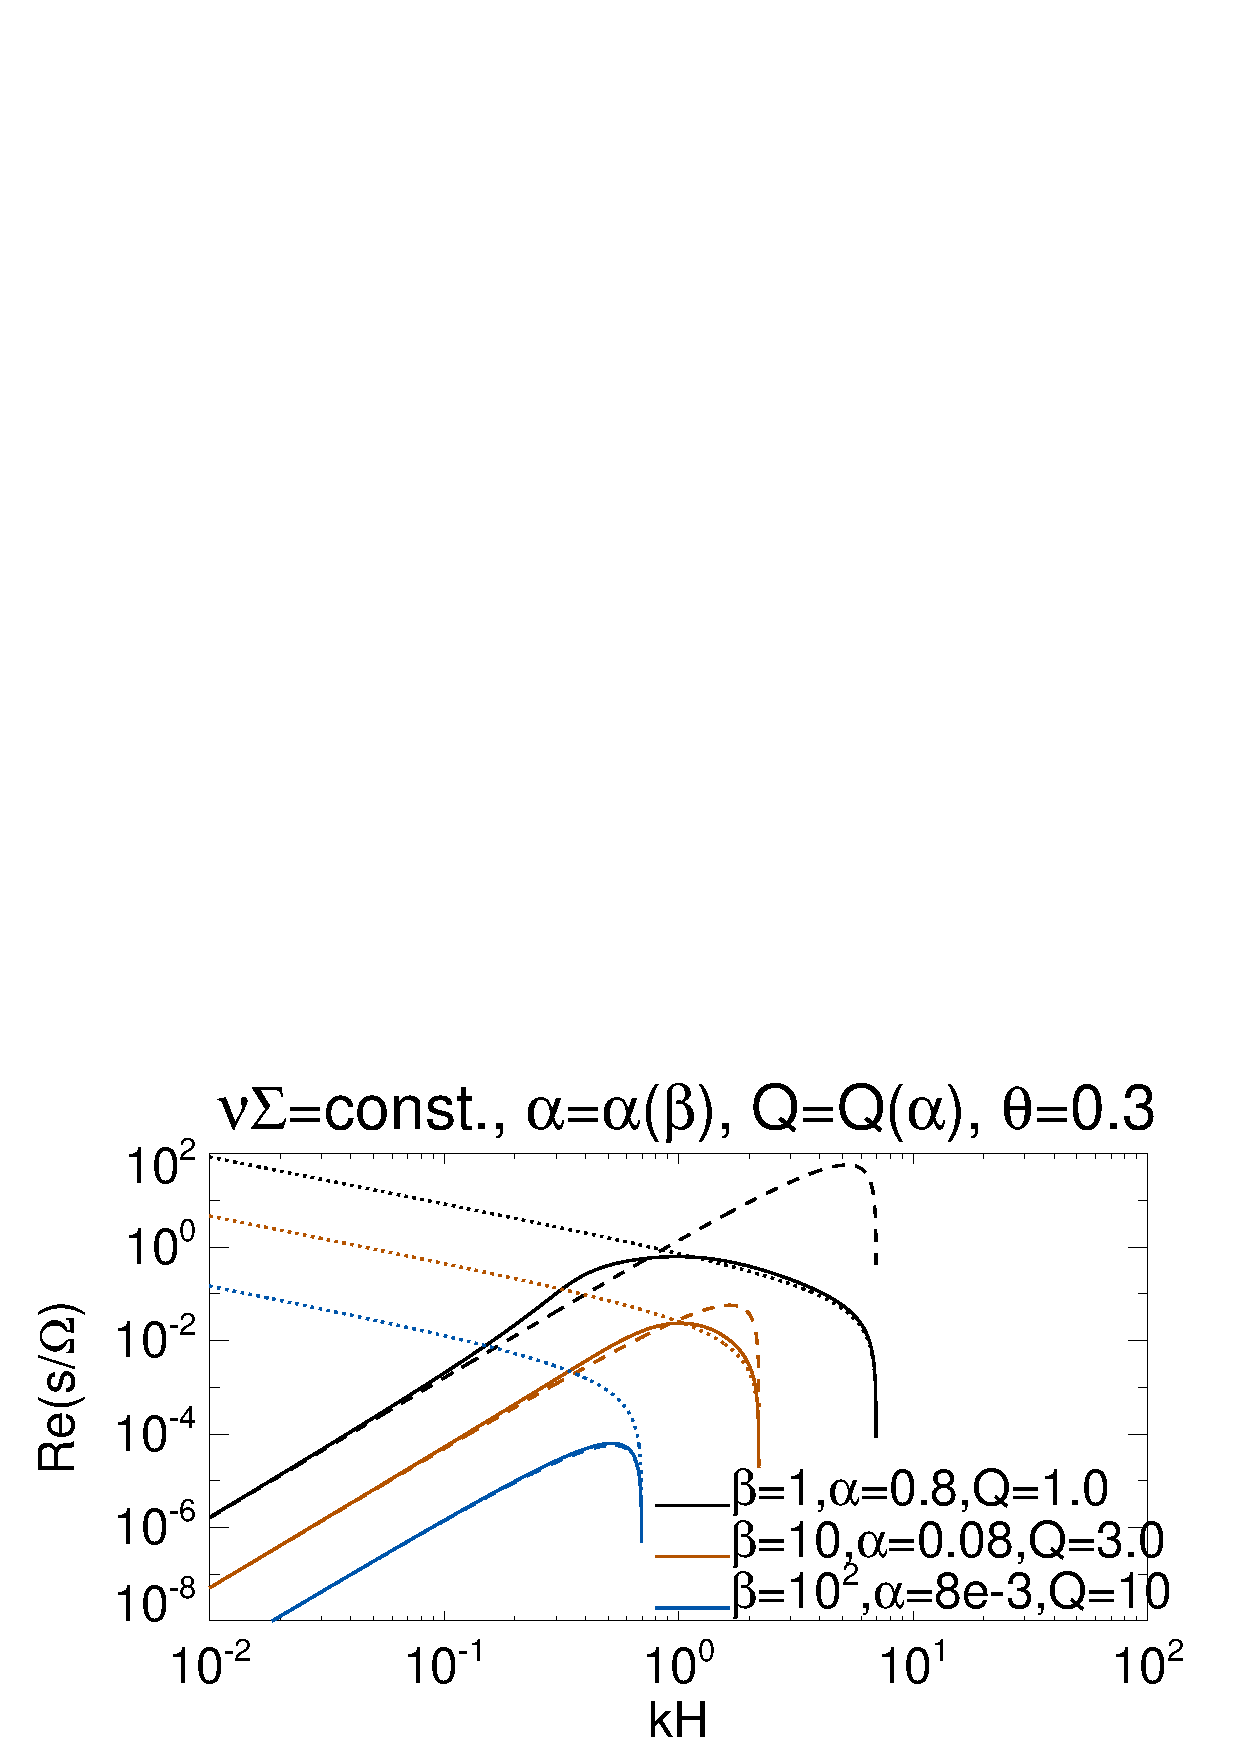
\includegraphics[width=\linewidth,clip=true,trim=0cm 0cm 0.4cm
    0.0cm]{figures/viscsg_modes_theta0d3}
  \caption{Growth rates for the 2D viscous problem as a function of
    the radial wavenumber $k$ for a range of cooling times
    $\beta$. The dashed and dotted lines correspond to asympototic
    behaviors for small and large $k$, respectively, computed from
    Eq. \ref{gammie_smallk} and \ref{gammie_bigk}. Top: without
    irradiation, bottom: partially irradiated disk. 
    \label{gammie_rate_plot}}
\end{figure}


Fig. \ref{gammie_maxrate_plot} shows the maximum
growth rate (top panel) and the corresponding wavenumber (bottom
panel) as a function of the cooling time $\beta$ for $\theta=0$.  
There is good agreement between numerical growth rates and
Eq. \ref{gammie_maxrate_simple} for $\beta \gtrsim 1$. 
%The assumption
%of $|\beta S|\ll 1$ is not well satisfied at smaller $\beta$ which
%explains the mismatch there. 
Eq. \ref{gammie_maxrate_simple} gives the
limiting behavior for this case as   
\begin{align*}
  S_*\propto \begin{cases}
%    \frac{\alpha^{1/4}}{Q\beta^{3/4}} \propto \beta^{-3/2} 
    \alpha^{1/4}\beta^{-3/4}Q^{-1}\propto \beta^{-3/2} 
    &  \beta \gg \alpha, \\
%    \frac{1}{Q\sqrt{\alpha}}  
    \alpha^{-1/2}Q^{-1} = \mathrm{const.} & \beta \ll \alpha,    
  \end{cases}
\end{align*}
where we have applied Eq. \ref{alpha_beta_relation}
and \ref{Qalpha}. The disk is formally unstable for all $\beta$, but
growth timescales are long ($>10$ orbits) for $\beta \gtrsim
20$. This region is marked by the vertical dashed-dotted line in
Fig. \ref{gammie_maxrate_plot}. The optimum wavenumber decreases with
the cooling time for $\beta\lesssim O(1)$ because larger scales are
more resistant to the associated increase in viscous damping.      

{\bf maybe move following to discussion}
Numerical simulations of self-gravitating disks show there is a
maximum $\alpha$ ($\sim 0.06$) that can be sustained before
fragmentation \citep{rice11}. We can interpret this result in our
linear framework. 
%We can use our case (\ref{gvisc}) to interpret this
Suppose it is possible to balance rapid cooling ($\beta\lesssim1$) 
by generating a large gravito-turbulent heating rate
($\alpha\gtrsim 1$) through a small $Q$. Fig. \ref{gammie_maxrate_plot} 
shows that such a system would be dynamically unstable with 
growth rate $s = O(\Omega)$. This due to the direct effect of viscous 
stress promoting instability, rather than cooling. Thus, we do not expect rapidly-cooled, 
and hence highly turbulent, self-gravitating disks to persist beyond
dynamical timescales. This is consistent with previous numerical
simulations performed by \cite{lodato05}. 
%Case (\ref{gvisc}) is consistent with 
\begin{figure}
%  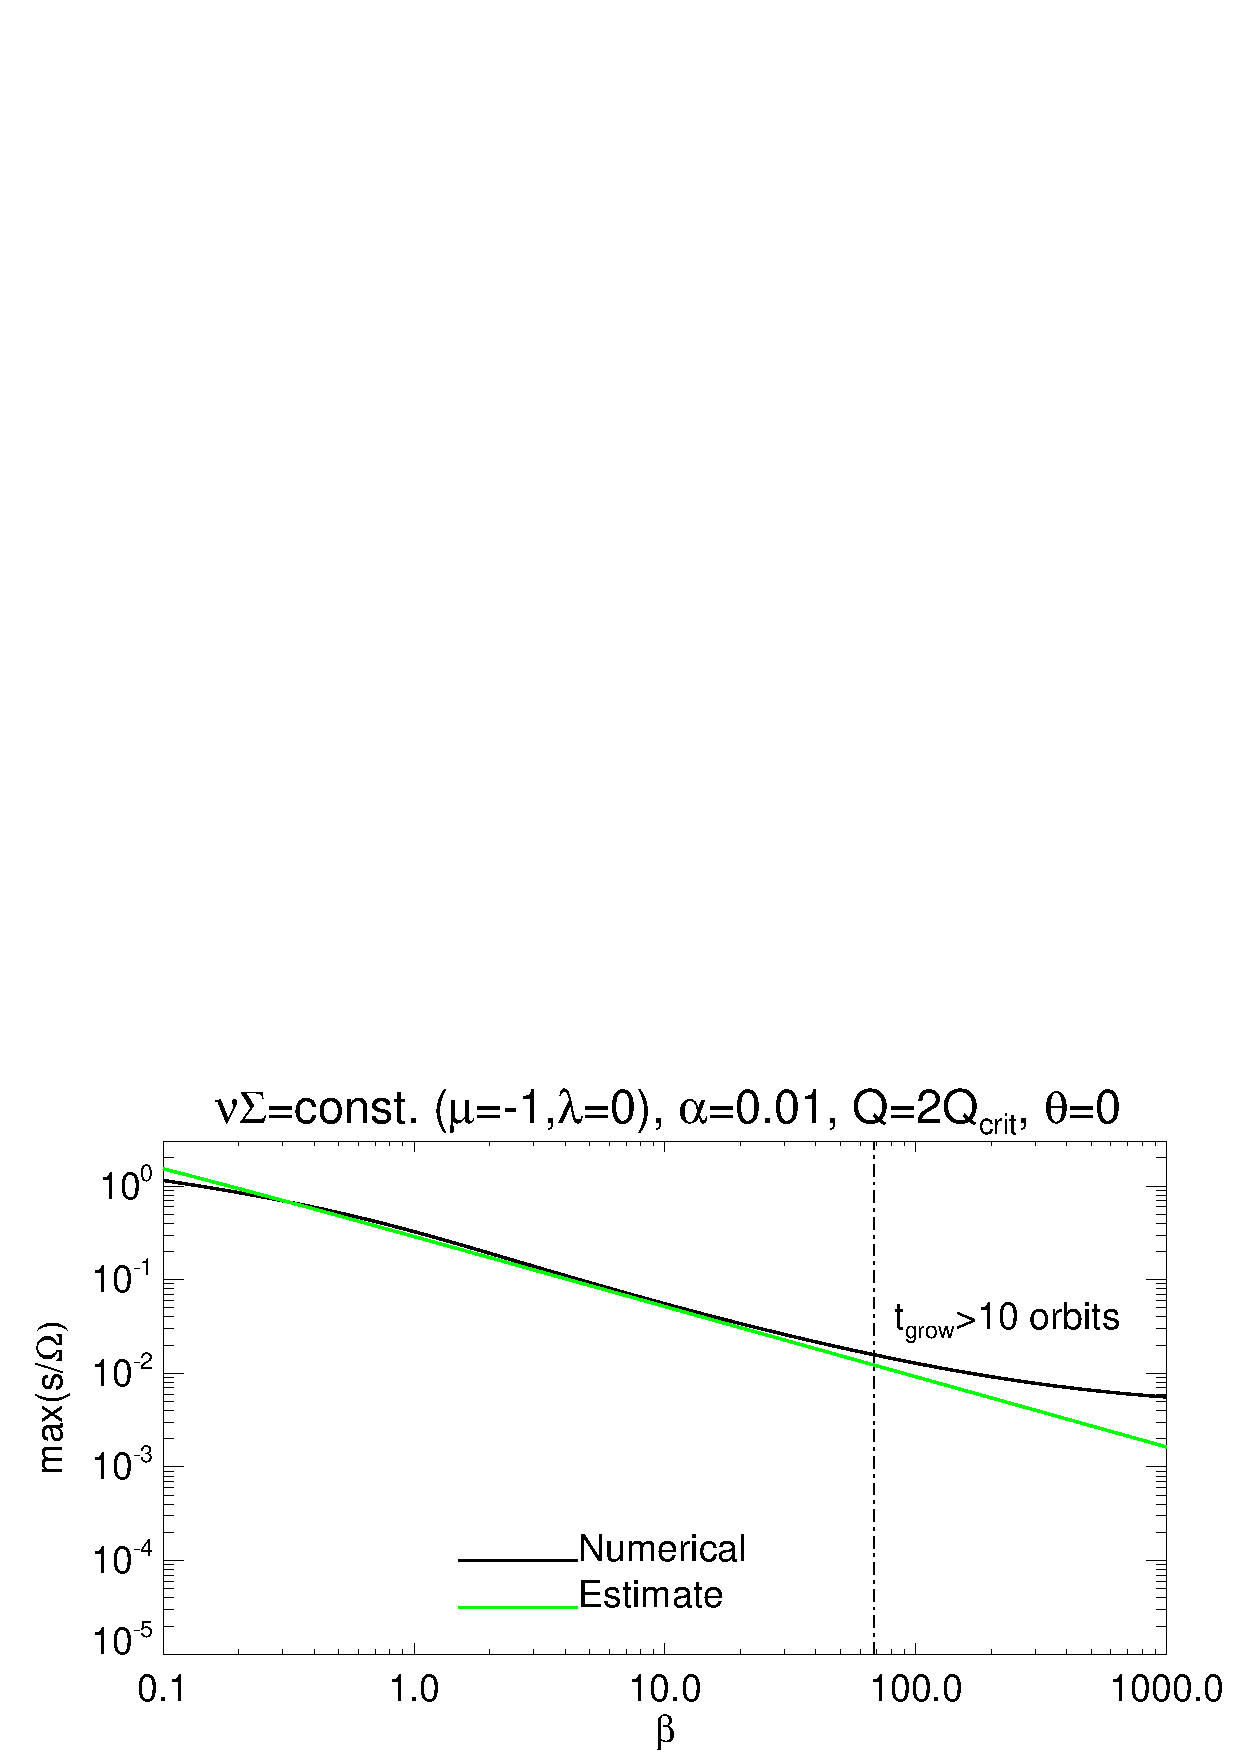
\includegraphics[width=\linewidth,clip=true,trim=0cm 1.5cm 0cm
%    0.0cm]{figures/result2d_fixalpha}\\
%  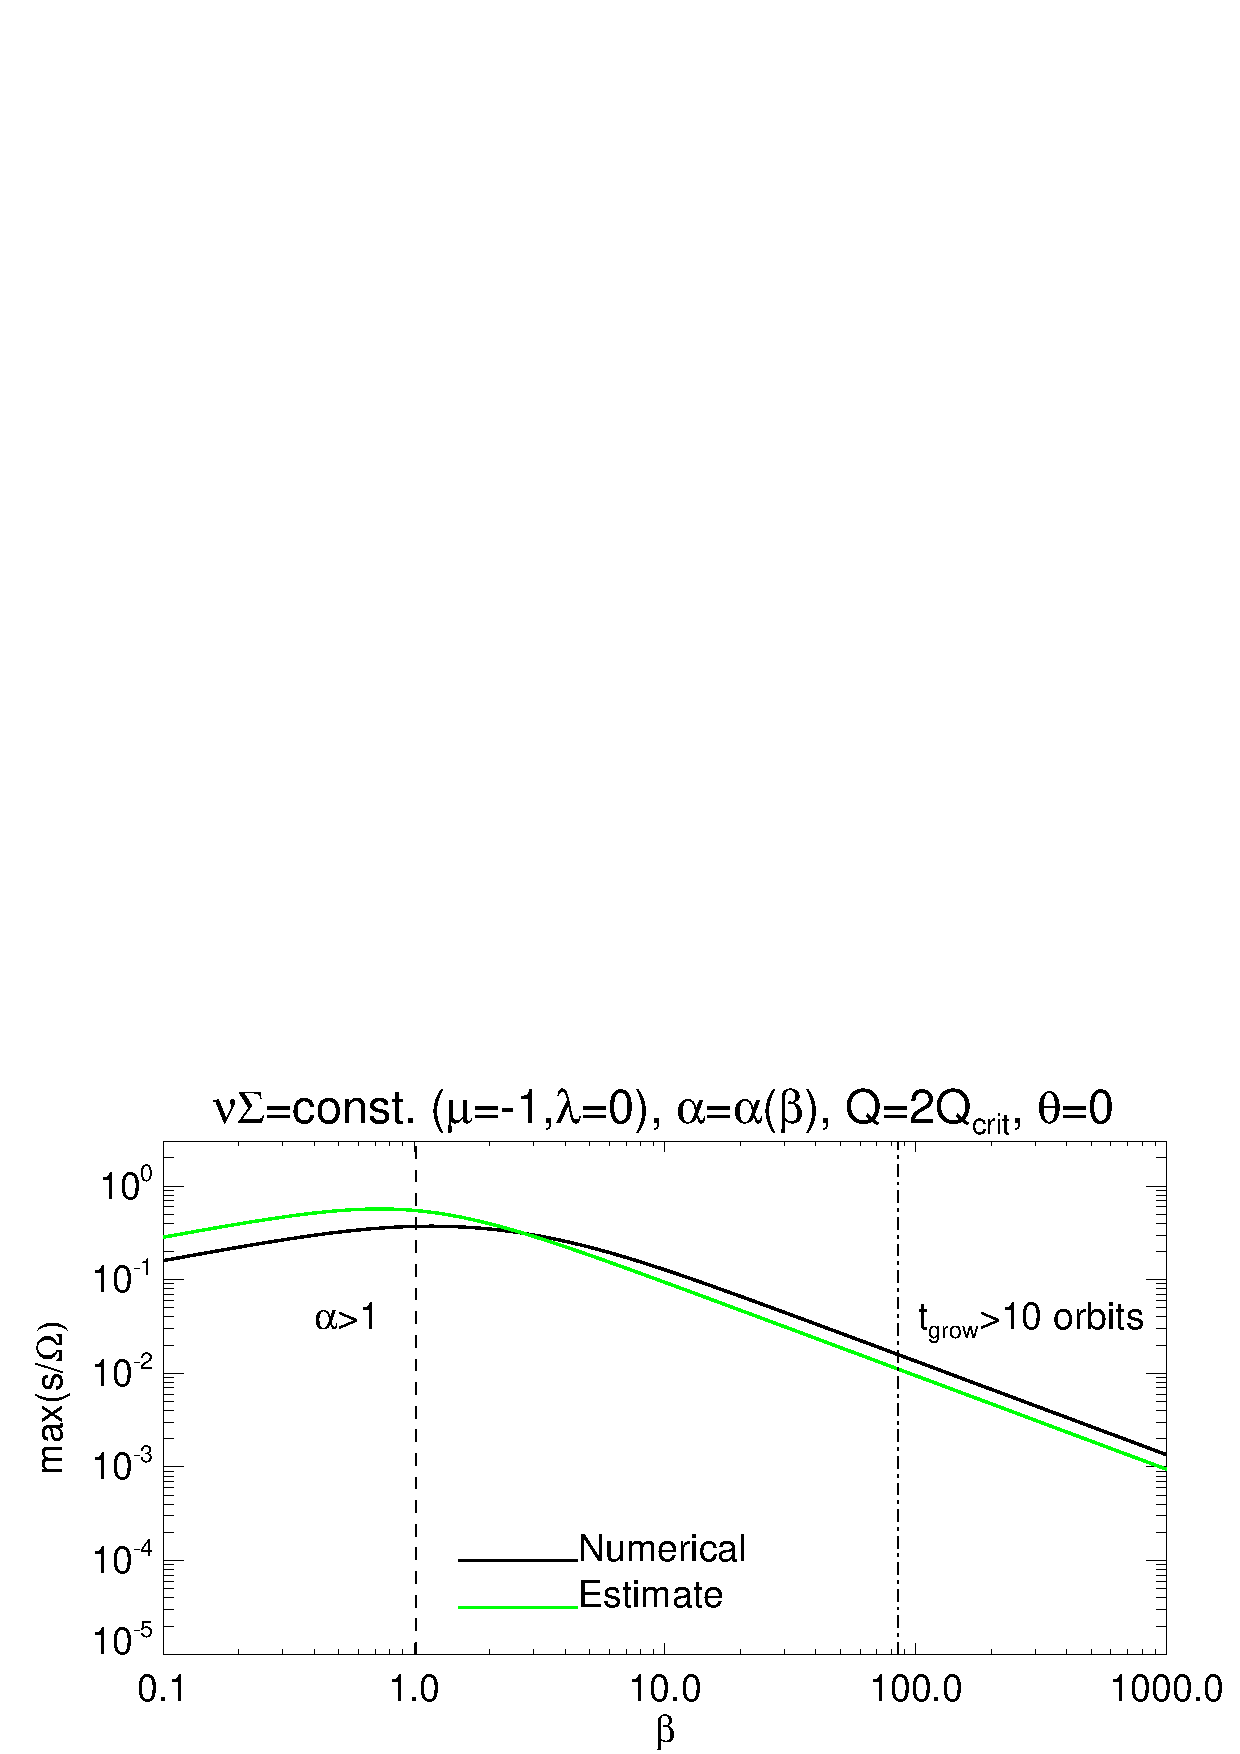
\includegraphics[width=\linewidth,clip=true,trim=0cm 1.5cm 0cm
%    0.0cm]{figures/result2d_fixQ}\\
  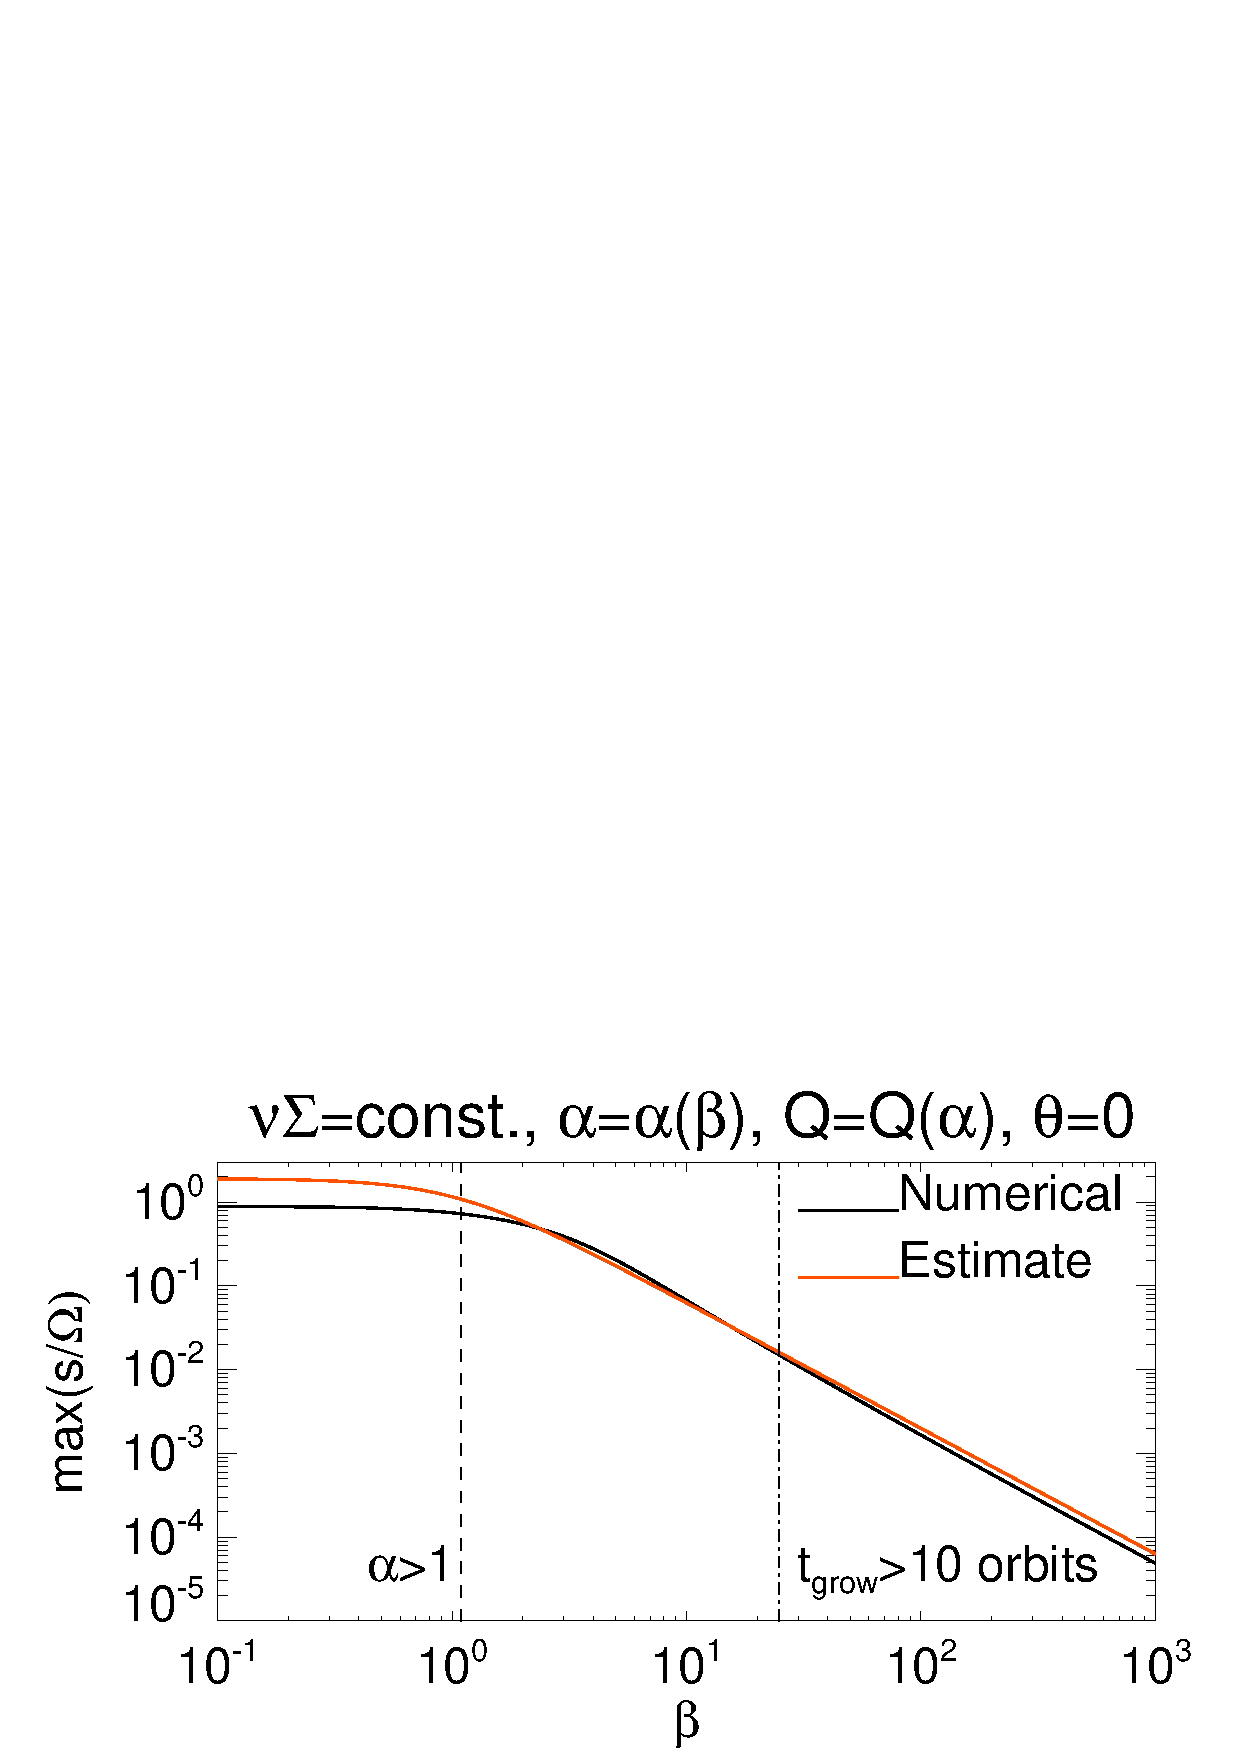
\includegraphics[width=\linewidth,clip=true,trim=0cm 1.5cm 0.cm
    0.0cm]{figures/result2d_gvisc}
  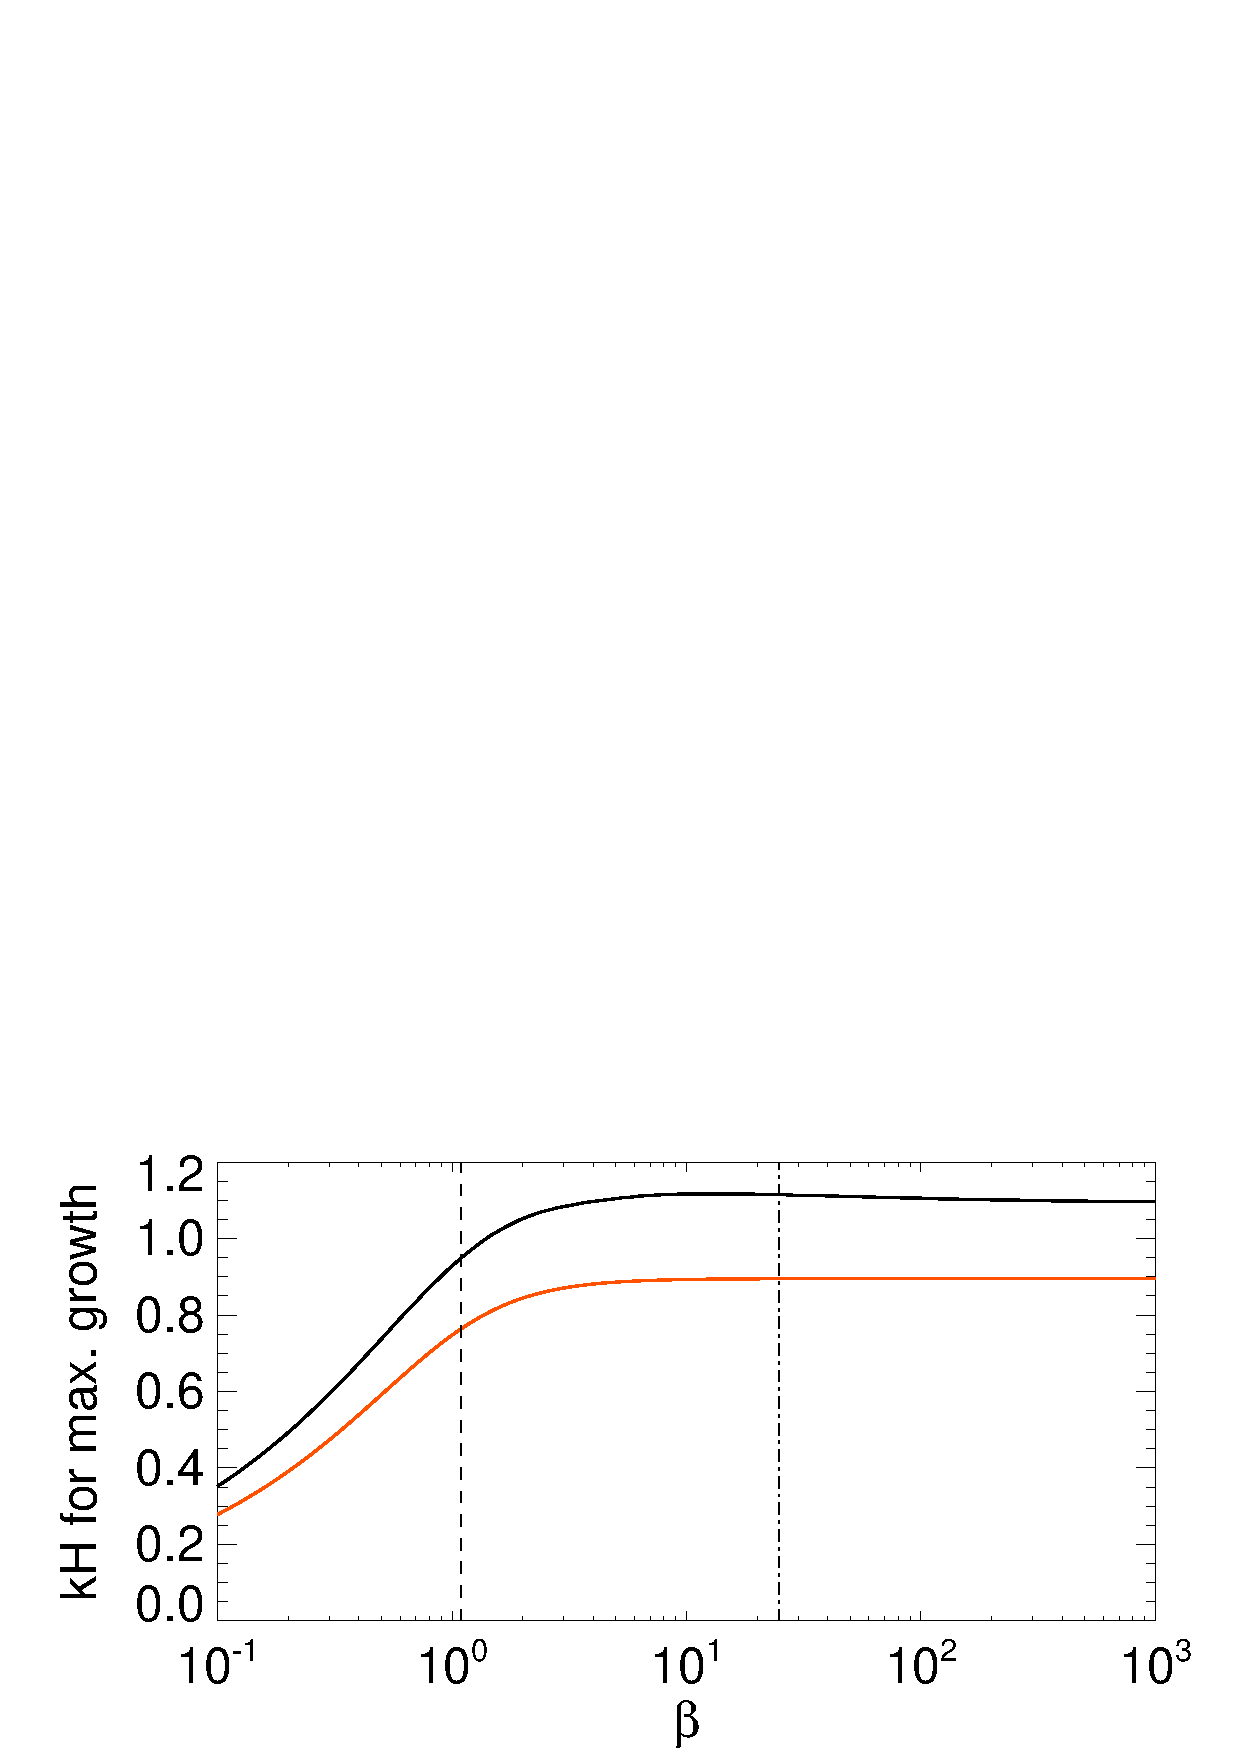
\includegraphics[width=\linewidth,clip=true,trim=0cm 0cm 0.cm
    1.0cm]{figures/result2d_gvisc_kmax}
  \caption{Growth rates (top) at the optimal wavenumber (bottom) for
    viscous GI as a function of cooling time for the
    case shown in Fig. \ref{gammie_rate_plot}. Solid lines are
    computed from the dispersion relation (Eq. \ref{thindisk}), and the dotted line is an
    estimate from Eq. \ref{gammie_maxrate_simple}. The vertical dashed
    line marks the region with $\alpha > 1$, and the vertical
    dashed-dot line marks the region with growth timescales longer
    than dynamical. 
    \label{gammie_maxrate_plot}}
\end{figure}
